\hsection{Cloning git Repositories under Pycharm}%
\label{sec:gitClonePycharm}%
%
\begin{figure}%
\centering%
%
\subfloat[][%
Maybe we find an interesting repository on \github. %
Let's say it is \url{\databasesCodeRepo}. %
We click on the \menu{Code} drop down menu.%
\label{fig:gitClonePycharm01website}%
]{\tightbox{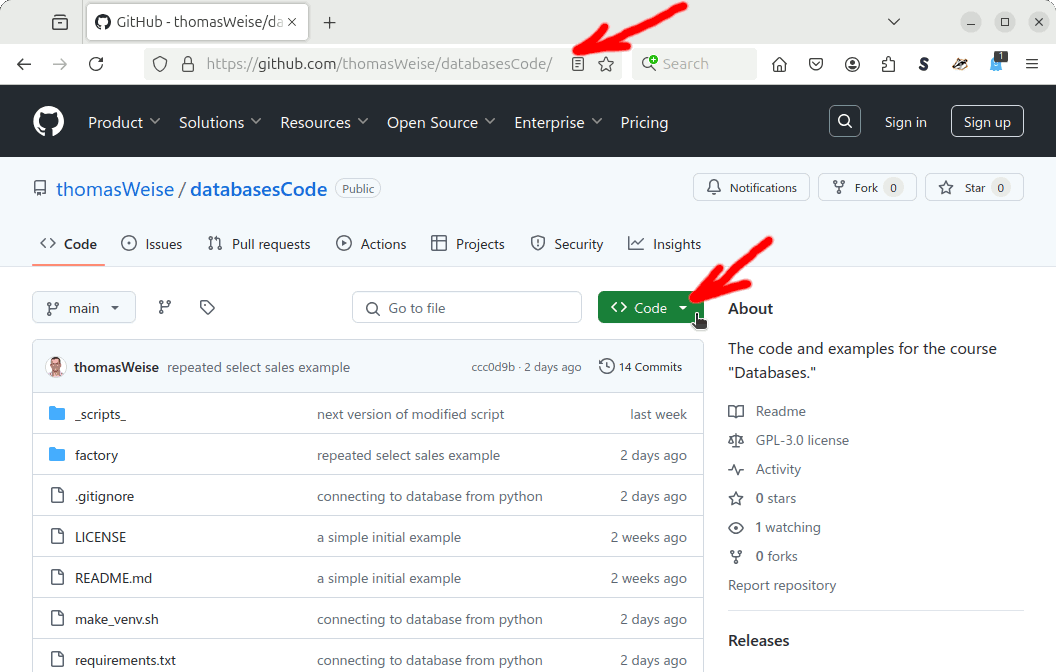
\includegraphics[width=0.78\linewidth]{\currentDir/gitClonePycharm01website}}}%
%
\floatRowSep%
%
\subfloat[][%
We click on the button for copying the \pgls{URL} to the clipboard.%
\label{fig:gitClonePycharm02copyUrl}%
]{\tightbox{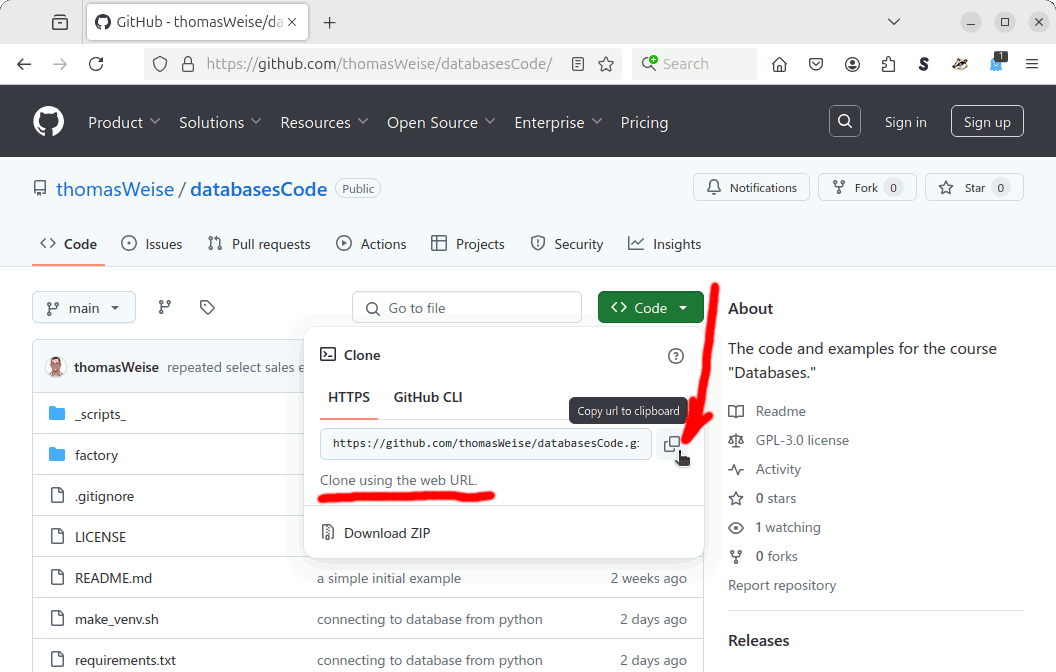
\includegraphics[width=0.48\linewidth]{\currentDir/gitClonePycharm02copyUrl}}}%
%
\floatSep%
%
\subfloat[][%
Now the \pgls{URL} is copied to the clipboard and we can paste it wherever we like via~\keys{\ctrl+V}.%
\label{fig:gitClonePycharm03copiedUrl}%
]{\tightbox{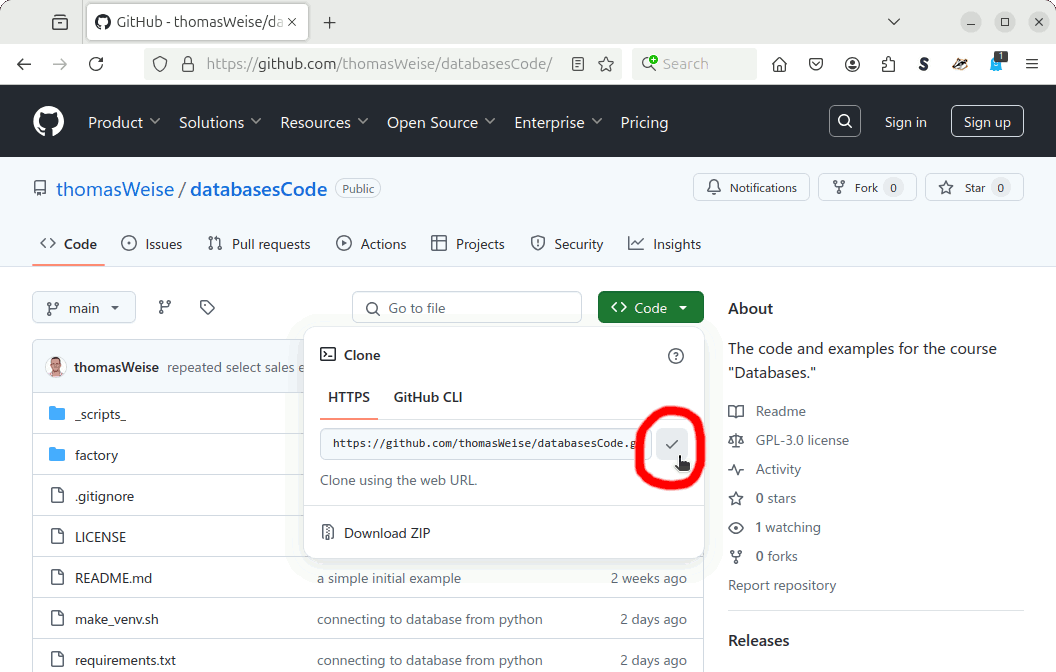
\includegraphics[width=0.48\linewidth]{\currentDir/gitClonePycharm03copiedUrl}}}%
%
\floatRowSep%
%
\subfloat[][%
We open \pycharm. If we get to the \emph{Welcome to \pycharm} screen, we click \menu{Clone Repository}.%
\label{fig:gitClonePycharm04AcloneRepository}%
]{\tightbox{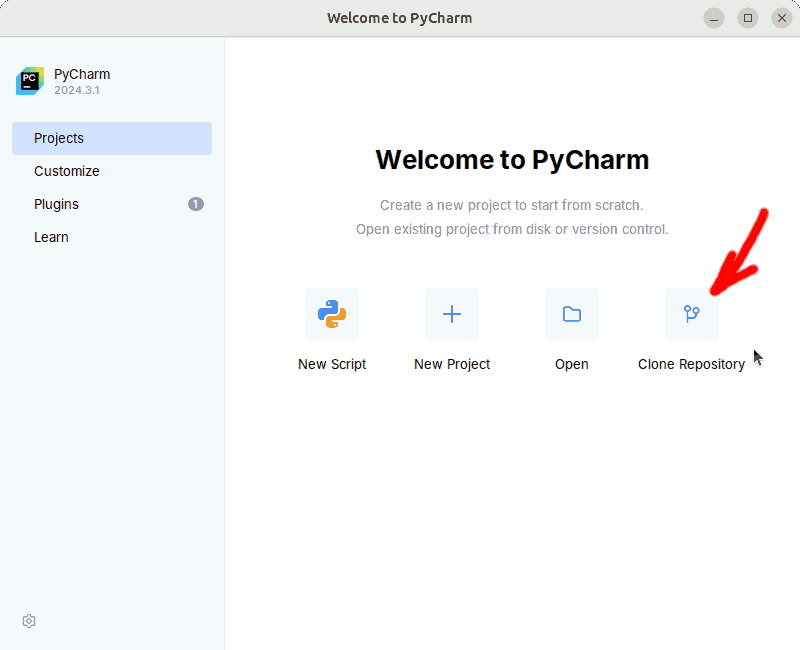
\includegraphics[width=0.48\linewidth]{\currentDir/gitClonePycharm04AcloneRepository}}}%
%
\floatSep%
%
\subfloat[][%
If we already have a project open in \pycharm, we click on \menu{\pycharmMainMenu > File > Project from Version Control\dots}.%
\label{fig:gitClonePycharm04BcloneRepository}%
]{\tightbox{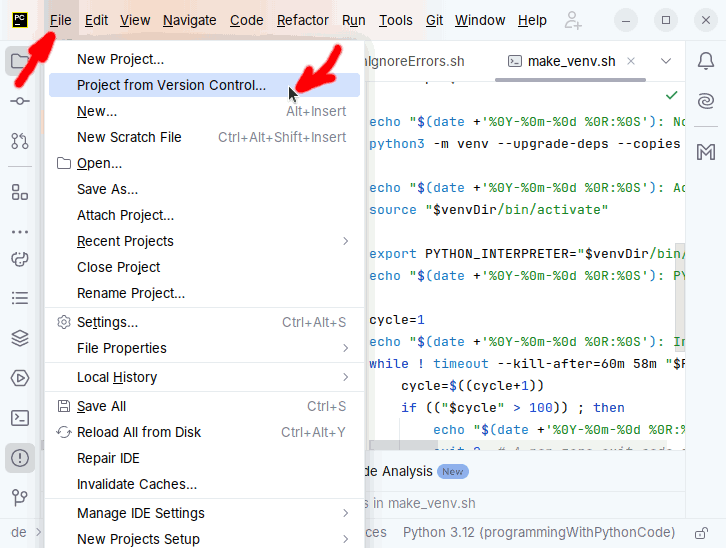
\includegraphics[width=0.48\linewidth]{\currentDir/gitClonePycharm04BcloneRepository}}}%
%
\caption{Cloning a \git\ (or \github) repository in \pycharm\ and configuring a \pgls{virtualEnvironment} for it.}%
\label{fig:gitClonePycharmA}%
\end{figure}%
%
\begin{figure}%
\ContinuedFloat%
\centering%
%
\subfloat[][%
The \inQuotes{Clone Repository} form appears.%
\label{fig:gitClonePycharm05cloneRepositoryForm}%
]{\tightbox{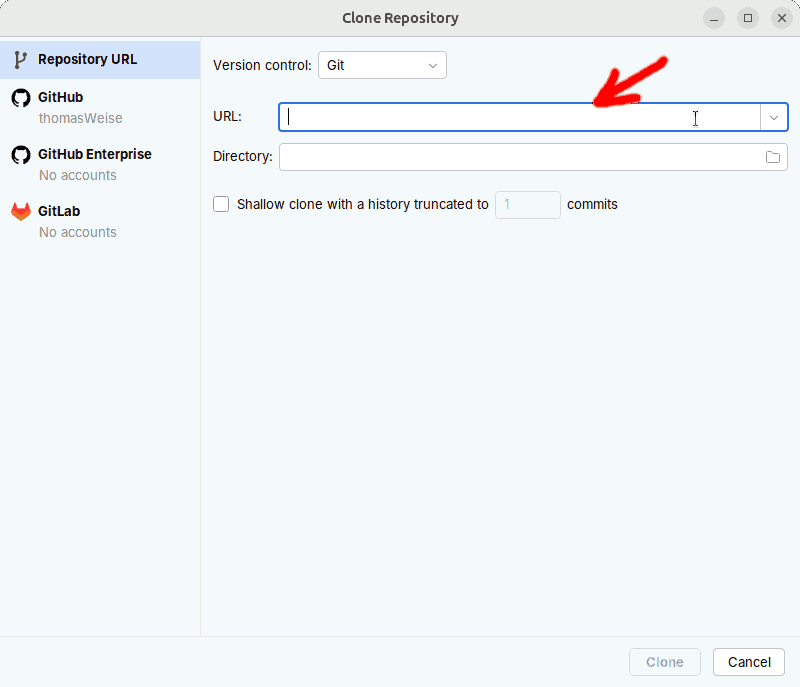
\includegraphics[width=0.48\linewidth]{\currentDir/gitClonePycharm05cloneRepositoryForm}}}%
%
\floatSep%
%
\subfloat[][%
Normally, we would write the \pgls{URL} of the repository that we want to clone into the \menu{URL:} field. %
Here, we paste the repository \pgls{URL} that we copied from the \github\ page with \keys{\ctrl + V}. %
We also enter a directory where the repository should be copied to into the \menu{Directory:} field. %
Here, I simply selected a folder on my \linux\ temporary files partition (because I will delete the project once I am done with this example). %
You would instead choose a more appropriate location. %
Then we click~\menu{Clone}.%
\label{fig:gitClonePycharm06cloning}%
]{\tightbox{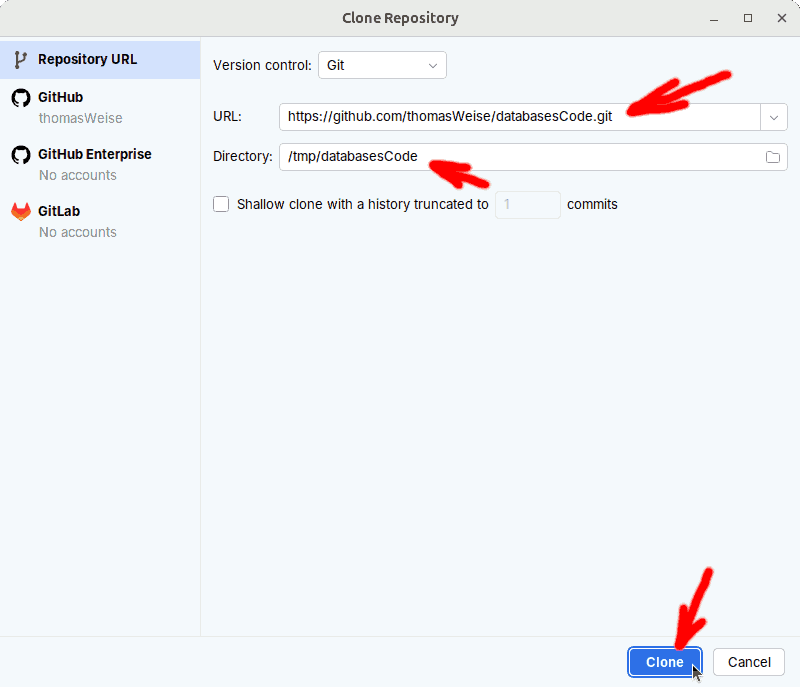
\includegraphics[width=0.48\linewidth]{\currentDir/gitClonePycharm06cloning}}}%
%
\floatRowSep%
%
\subfloat[][%
The download will begin. %
We may get asked whether we want to trust the downloaded project. %
If and only if we do trust it, we click~\menu{Trust Project}.%
\label{fig:gitClonePycharm07trustQuestion}%
]{\tightbox{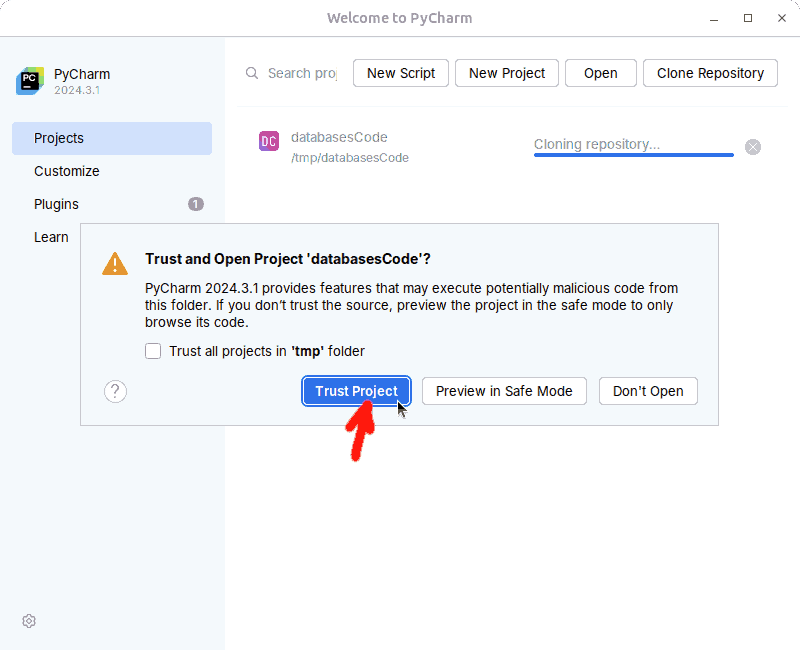
\includegraphics[width=0.48\linewidth]{\currentDir/gitClonePycharm07trustQuestion}}}%
%
\floatSep%
%
\subfloat[][%
The repository is downloaded and opens as new project in \pycharm. %
If this is a \python\ project, we now can configure its \pgls{virtualEnvironment} settings (see \cref{sec:venvAndPycharm}). %
To do so, we click on \keys{\pycharmMainMenu}.%
\label{fig:gitClonePycharm08open}%
]{\tightbox{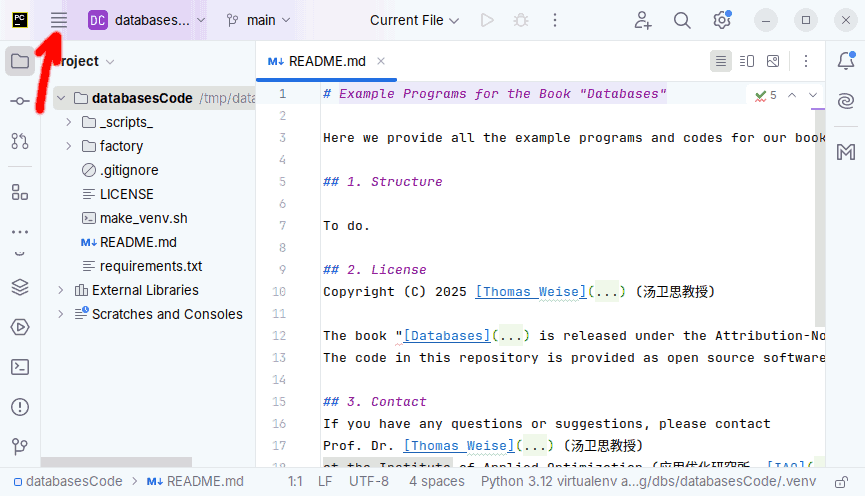
\includegraphics[width=0.48\linewidth]{\currentDir/gitClonePycharm08open}}}%
%
\caption{Cloning a \git\ (or \github) repository in \pycharm\ and configuring a \pgls{virtualEnvironment} for it.}%
\label{fig:gitClonePycharmB}%
\end{figure}%
%
\begin{figure}%
\ContinuedFloat%
\centering%
%
\subfloat[][%
In the menu that opens, we click on \menu{Settings\dots}~(we could also press \keys{\ctrl+\Alt+S}).%
\label{fig:gitClonePycharm09settings}%
]{\tightbox{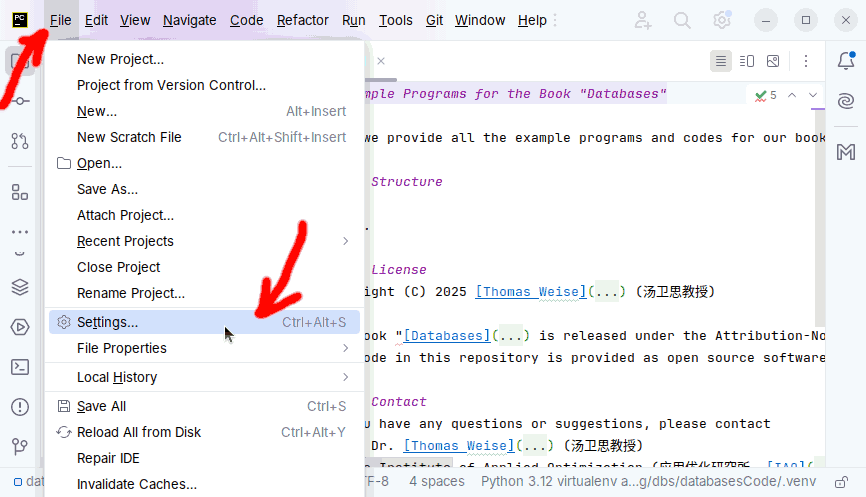
\includegraphics[width=0.48\linewidth]{\currentDir/gitClonePycharm09settings}}}%
%
\floatSep%
%
\subfloat[][%
The \menu{Settings} menu opens. %
In the pane on the left-hand side, we click on the item \menu{Project: \inQuotes{our project}} and then on \menu{Python Interpreter}. %
This shows us something like the view on the left hand side: Maybe the system \python\ interpreter is selected or something else. %
We want to set up a \pgls{virtualEnvironment} for our project, so we click on~\menu{Add Interpreter}.%
\label{fig:gitClonePycharm10interpreter}%
]{\tightbox{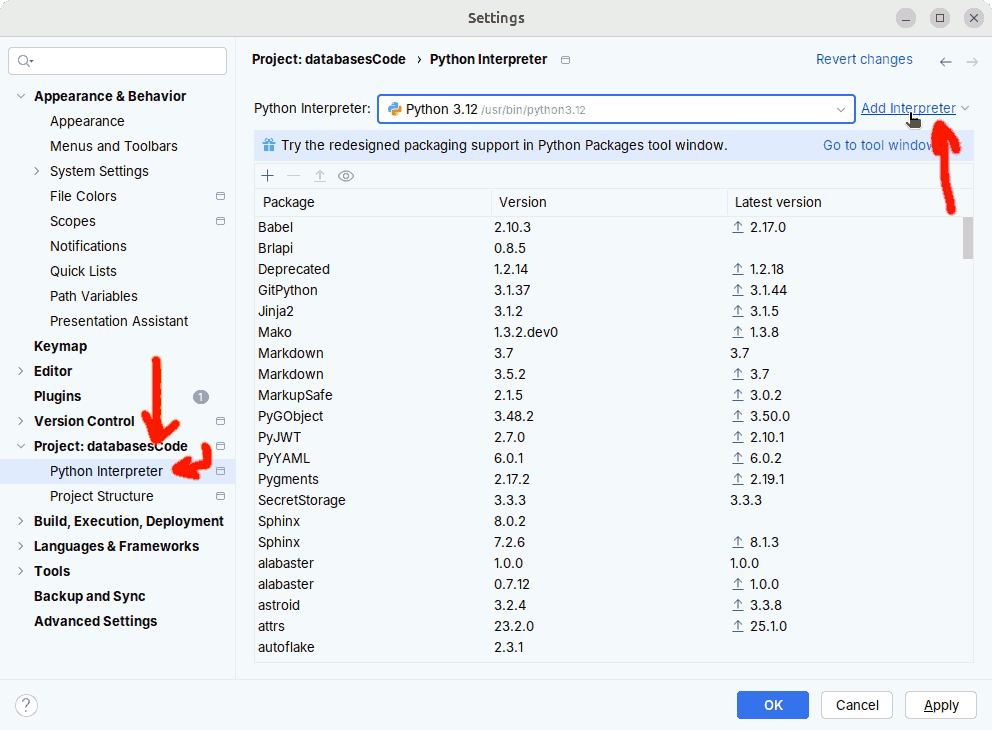
\includegraphics[width=0.48\linewidth]{\currentDir/gitClonePycharm10interpreter}}}%
%
\floatRowSep%
%
\subfloat[][%
We then click on \menu{Add Local Interpreter}.%
\label{fig:gitClonePycharm11addLocal}%
]{\tightbox{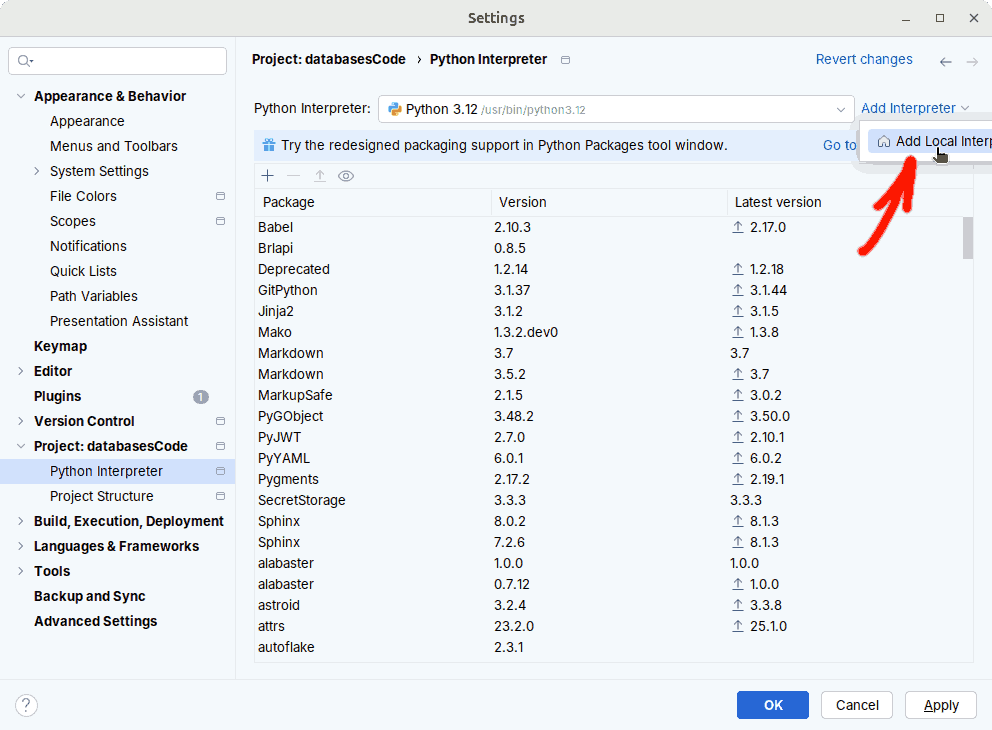
\includegraphics[width=0.48\linewidth]{\currentDir/gitClonePycharm11addLocal}}}%
%
\floatSep%
%
\subfloat[][%
In the \inQuotes{Add Python Interpreter} dialog that opens up, we select \menu{Generate New}, choose \menu{Virtualenv}, and type the sub-directory \textil{.venv} relative to the path where we cloned the repository into as \menu{Location:}. %
We then click~\menu{OK}.%
\label{fig:gitClonePycharm12addNew}%
]{\tightbox{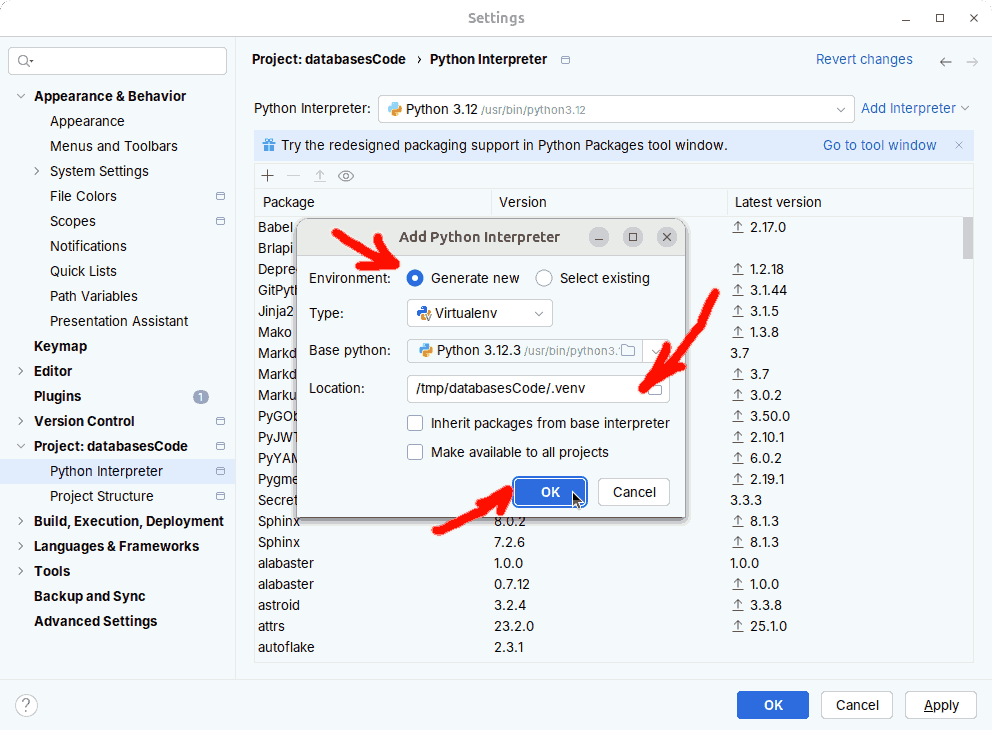
\includegraphics[width=0.48\linewidth]{\currentDir/gitClonePycharm12addNew}}}%
%
\floatRowSep%
%
\subfloat[][%
The new environment is created and we click on \menu{OK}.%
\label{fig:gitClonePycharm13addOK}%
]{\tightbox{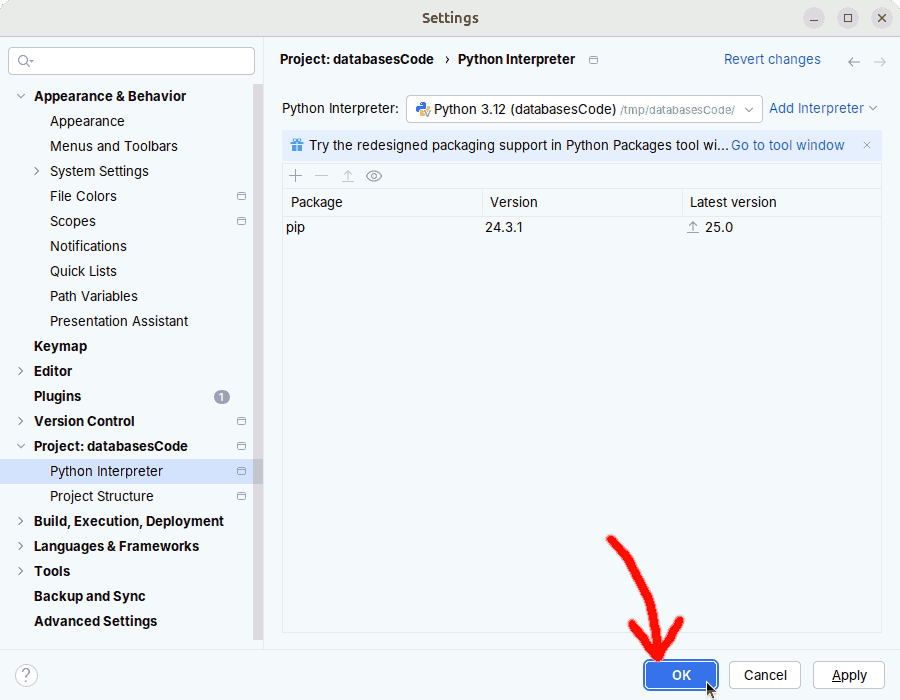
\includegraphics[width=0.48\linewidth]{\currentDir/gitClonePycharm13addOK}}}%
%
\floatSep%
%
\subfloat[][%
Indeed, a directory called \textil{.venv} appears in the directory view of our project.%
\label{fig:gitClonePycharm14added}%
]{\tightbox{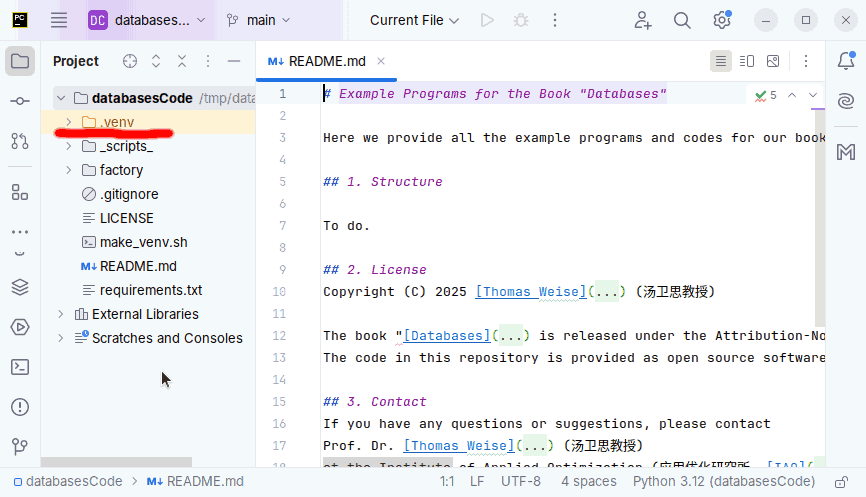
\includegraphics[width=0.48\linewidth]{\currentDir/gitClonePycharm14added}}}%
%
\caption{Cloning a \git\ (or \github) repository in \pycharm\ and configuring a \pgls{virtualEnvironment} for it.}%
\label{fig:gitClonePycharmC}%
\end{figure}%
%
\begin{figure}%
\ContinuedFloat%
\centering%
%
\subfloat[][%
Many \python\ projects come with a file \textil{requirements.txt} or \textil{requirements-dev.txt}. %
As discussed in \cref{sec:requirementsFiles}, these list the libraries that the projects depend on. %
Our example repository also has a file \textil{requirements.txt}, stating that it needs library~\psycopg. %
This dependency is marked with yellow color, because it is not installed in the \pgls{virtualEnvironment}.%
\label{fig:gitClonePycharm15requirements}%
]{\tightbox{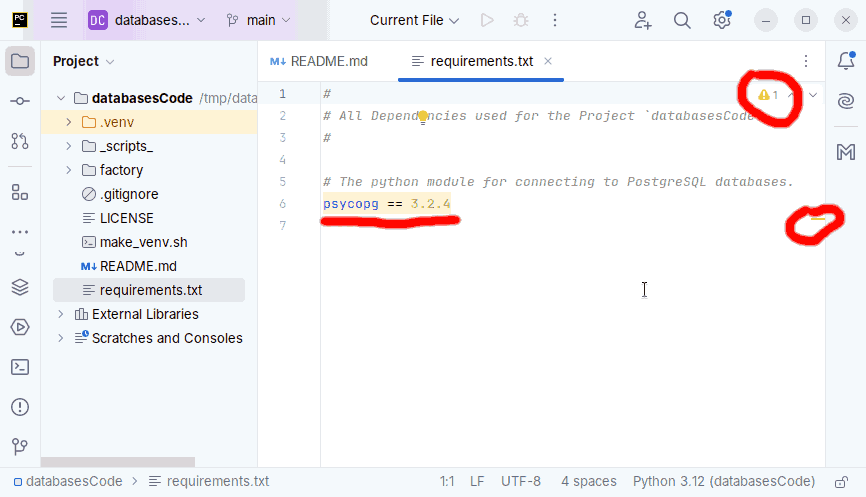
\includegraphics[width=0.48\linewidth]{\currentDir/gitClonePycharm15requirements}}}%
%
\floatSep%
%
\subfloat[][%
Clicking on the warnings symbol~\pycharmWarningsSymbol\ reveals this issue.%
\label{fig:gitClonePycharm16requirementsWarning}%
]{\tightbox{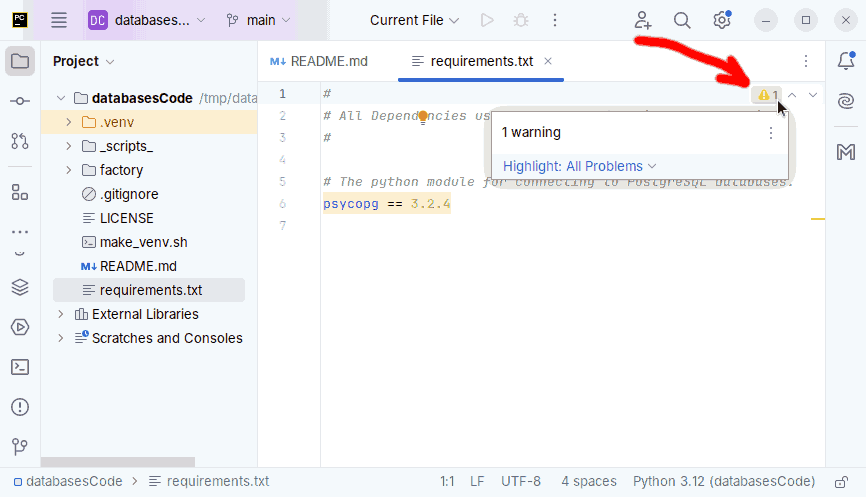
\includegraphics[width=0.48\linewidth]{\currentDir/gitClonePycharm16requirementsWarning}}}%
%
\floatRowSep%
%
\subfloat[][%
Indeed: If we look at the \textil{.venv} directory in the directory view, we cannot find the \psycopg\ package.%
\label{fig:gitClonePycharm17packageMissing}%
]{\tightbox{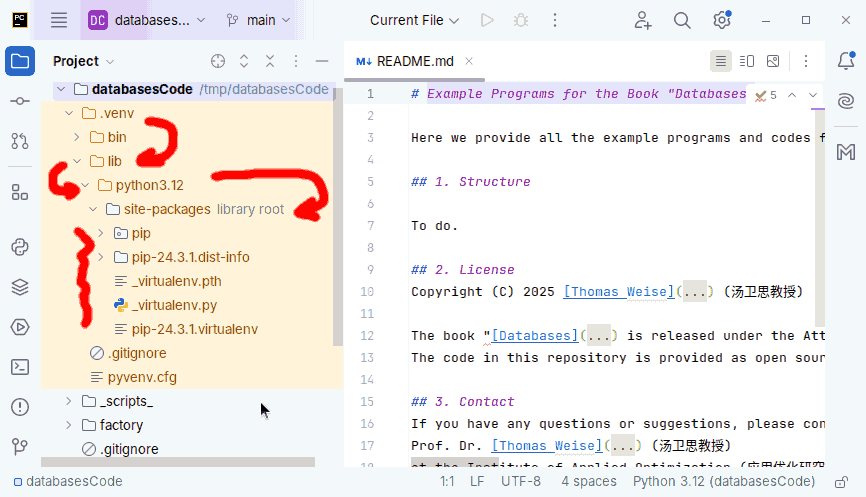
\includegraphics[width=0.48\linewidth]{\currentDir/gitClonePycharm17packageMissing}}}%
%
\floatSep%
%
\subfloat[][%
So we click on the requirements warning\dots%
\label{fig:gitClonePycharm18requirementsWarning}%
]{\tightbox{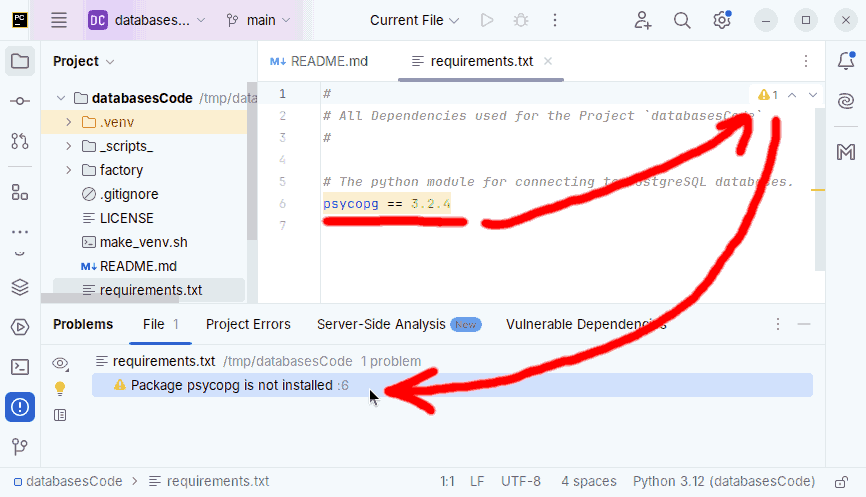
\includegraphics[width=0.48\linewidth]{\currentDir/gitClonePycharm18requirementsWarning}}}%
%
\floatRowSep%
%
\subfloat[][%
{\dots}and then on \menu{Show Quick-Fixes} (or press~\keys{\Alt+\enter}).%
\label{fig:gitClonePycharm19quickFixes}%
]{\tightbox{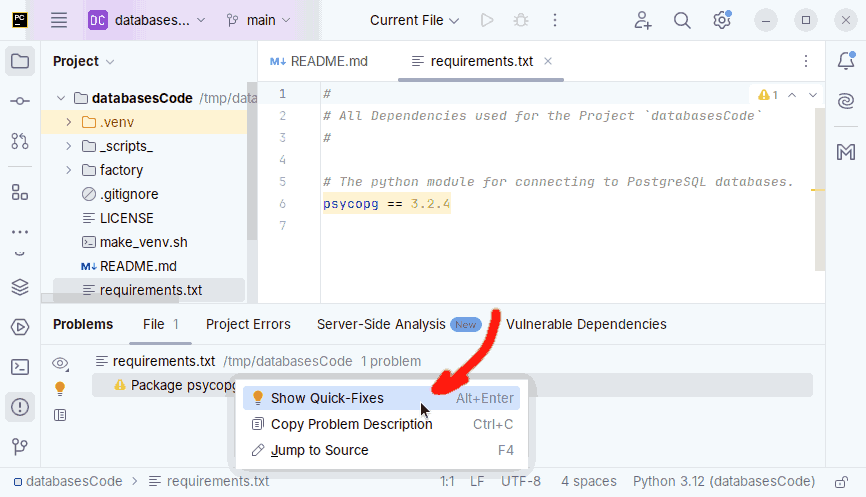
\includegraphics[width=0.48\linewidth]{\currentDir/gitClonePycharm19quickFixes}}}%
%
\floatSep%
%
\subfloat[][%
In the menu that opens up, we select~\menu{Install all missing packages}.%
\label{fig:gitClonePycharm20fixes}%
]{\tightbox{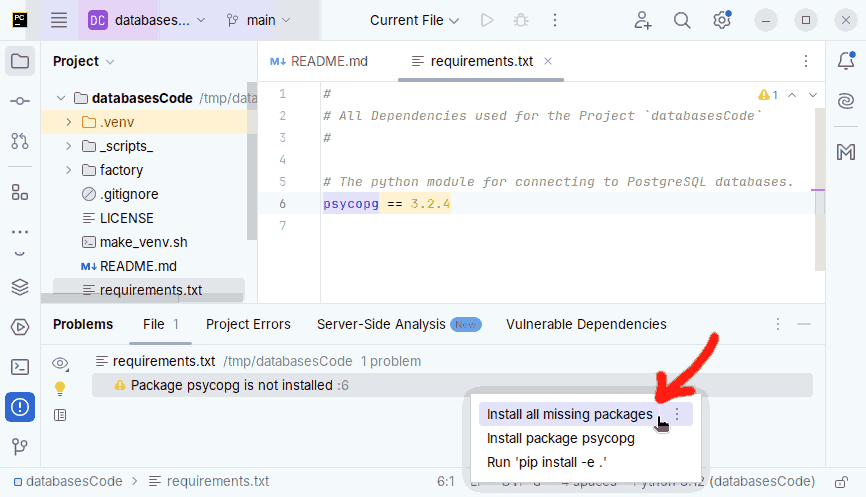
\includegraphics[width=0.48\linewidth]{\currentDir/gitClonePycharm20fixes}}}%
%
\caption{Cloning a \git\ (or \github) repository in \pycharm\ and configuring a \pgls{virtualEnvironment} for it.}%
\label{fig:gitClonePycharmD}%
\end{figure}%
%
\begin{figure}%
\ContinuedFloat%
\centering%
%
\subfloat[][%
We get presented a list of packages that will be installed. %
We click~\menu{OK}.%
\label{fig:gitClonePycharm21installAll}%
]{\tightbox{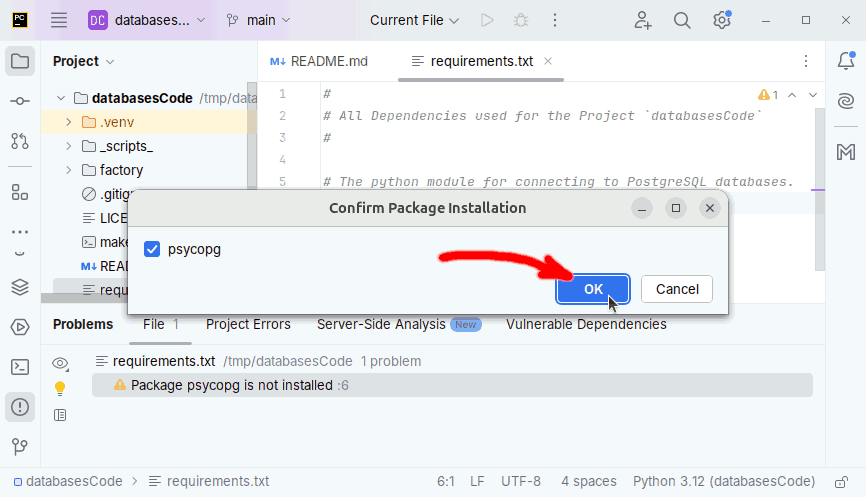
\includegraphics[width=0.48\linewidth]{\currentDir/gitClonePycharm21installAll}}}%
%
\floatSep%
%
\subfloat[][%
The required package(s) will now be downloaded and installed.%
\label{fig:gitClonePycharm22installing}%
]{\tightbox{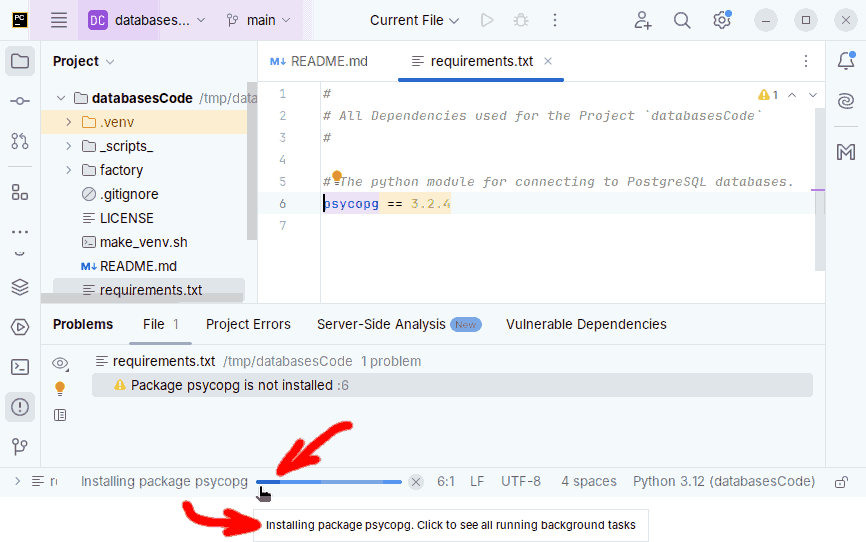
\includegraphics[width=0.48\linewidth]{\currentDir/gitClonePycharm22installing}}}%
%
\floatRowSep%
%
\subfloat[][%
The yellow warnings marks in the \textil{requirements.txt} file now disappear.%
\label{fig:gitClonePycharm23installed}%
]{\tightbox{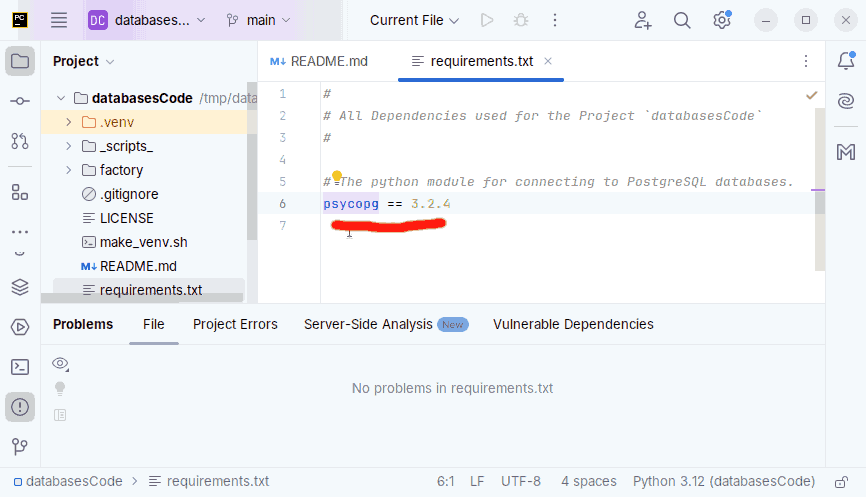
\includegraphics[width=0.48\linewidth]{\currentDir/gitClonePycharm23installed}}}%
%
\floatSep%
%
\subfloat[][%
And the packages have appeared in the \textil{.venv} directory as well.%
\label{fig:gitClonePycharm24installed}%
]{\tightbox{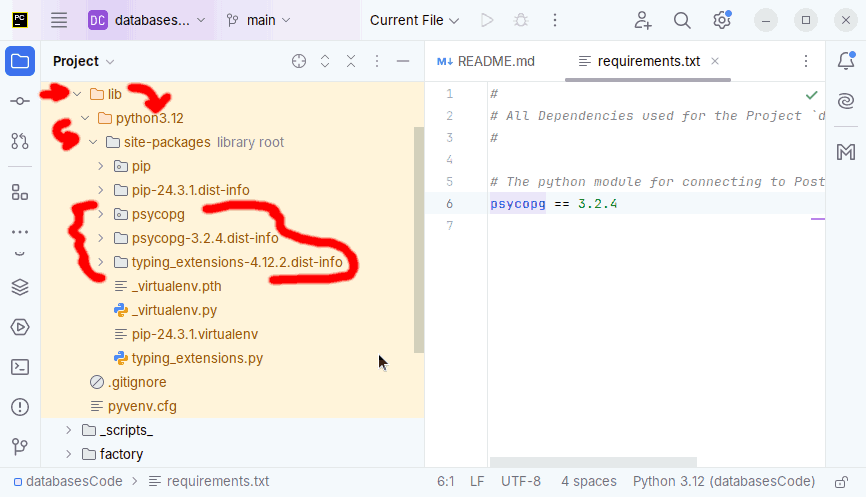
\includegraphics[width=0.48\linewidth]{\currentDir/gitClonePycharm24installed}}}%
%
\floatRowSep%
%
\subfloat[][%
All dependency packages are now installed. %
This means that the code in the repository that we have cloned will function now and we can run it.%
\label{fig:gitClonePycharm25run}%
]{\tightbox{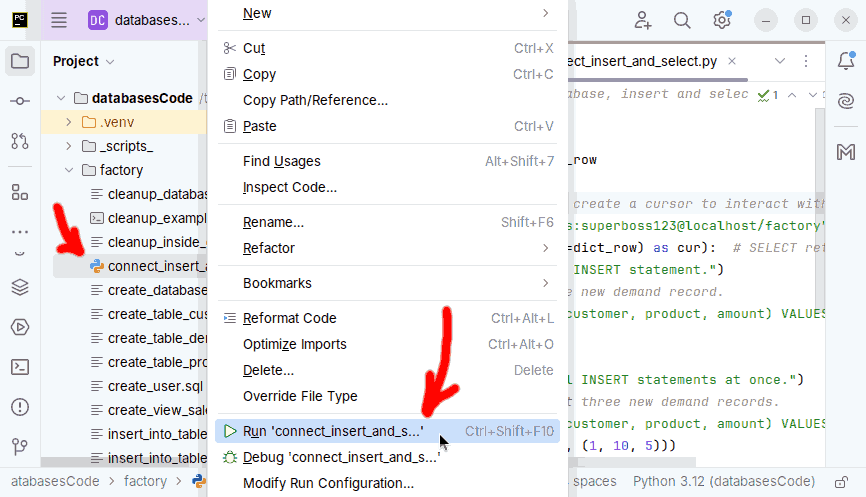
\includegraphics[width=0.48\linewidth]{\currentDir/gitClonePycharm25run}}}%
%
\caption{Cloning a \git\ (or \github) repository in \pycharm\ and configuring a \pgls{virtualEnvironment} for it.}%
\label{fig:gitClonePycharmE}%
\end{figure}%
%
\begin{figure}%
\ContinuedFloat%
\centering%
%
\subfloat[][%
Well, there may be other issues unrelated to packages{\dots} %
{\dots}the program I chose here is from our book on \citetitle{databases}~\cite{databases}, and it needs the \postgresql\ \pgls{dbms} running with a specific \pgls{db} ready. %
So likely, you cannot just run it {\dots} it was just an example.%
\label{fig:gitClonePycharm26ranError}%
]{\tightbox{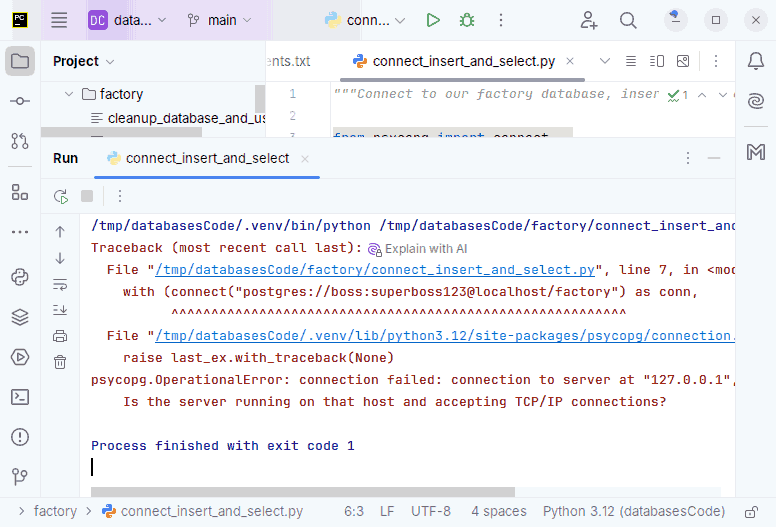
\includegraphics[width=0.48\linewidth]{\currentDir/gitClonePycharm26ranError}}}%
%
\floatSep%
%
\subfloat[][%
If you also follow the \citetitle{databases}~\cite{databases} course and have all other pieces of the software environment set up correctly, then you will see this output.%
\label{fig:gitClonePycharm26ranOK}%
]{\tightbox{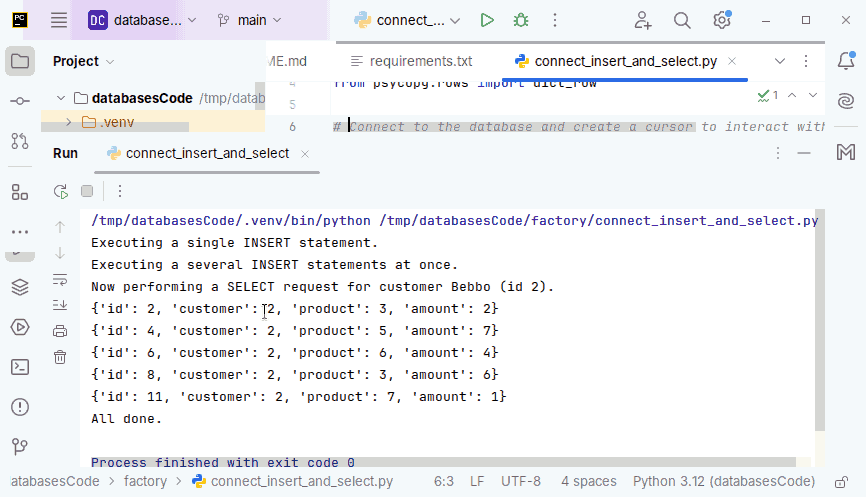
\includegraphics[width=0.48\linewidth]{\currentDir/gitClonePycharm26ranOK}}}%
%
\caption{Cloning a \git\ (or \github) repository in \pycharm\ and configuring a \pgls{virtualEnvironment} for it.}%
\label{fig:gitClonePycharmF}%
\end{figure}%
%
It is a very common scenario that we find an online repository with \python\ code that we are interested in.
Many papers in deep learning, for example, publish their code in this way.
Many such source code collections are \git\ repositories on \github.
The example programs that ship with this book~\cite{programmingWithPython} are published like this at \url{\programmingWithPythonCodeRepo}, for example.
We also have another book in progress, named \citetitle{databases}~\cite{databases}.
It, too, comes with a repository with sources for examples, this time at \url{\databasesCodeRepo}.

As usual, we work through a topic based on an example.
This time, our goal is to \emph{download and get to run code from a \github\ repository in \pycharm.}
Matter of fact, we already exercised the whole process of cloning the \github\ repository in \pycharm\ with the examples of this book in \cref{sec:gettingExamples}.
To complement the excursion from back then, we this time pick the companion code of our \citetitle{databases} book~\cite{databases} at \url{\databasesCodeRepo} as example.
This repository comes with a file \textil{requirements.txt}, which allows us to present the workflow of cloning a \git\ repository with setting up a \pgls{virtualEnvironment} and installing required packages into one single example.

Therefore, in \cref{fig:gitClonePycharm01website}, we pretend that you came across this interesting repository on \github\ using your normal web browser.
If you visit \url{\databasesCodeRepo}, you can see the big drop down menu~\menu{Code}.
If you click on it, it shows the \pgls{HTTPS} \pgls{URL} under which the project can be found in \cref{fig:gitClonePycharm02copyUrl}.
If you work with \github, there are two ways to write a \pgls{URL} to a repository:%
%
\begin{itemize}%
%
\item \url{https://github.com/user/repository} (or \url{https://github.com/user/repository.git}) use \gls{HTTPS} protocol to access the repository \textil{repository} of user \textil{user}. %
This form is often and commonly used.%
%
\item \url{ssh://git@github.com/user/repository} (or \url{ssh://git@github.com/user/repository.git}) use the \gls{SSH} to access the repository \textil{repository} of user \textil{user}. %
I find this form more reliable when working with \github\ from China. %
However, it requires an \pgls{SSH} key to be configured for authentication~\cite{GH2025ADCTGWS}.%
%
\end{itemize}%
%
Here, obviously, \textil{user} is \textil{thomasWeise}, which is my personal \github\ account, and \textil{repository} is \textil{databasesCode}.
The \pgls{URL} that will be copied to the clipboard by clicking the button in \cref{fig:gitClonePycharm02copyUrl} is \url{\databasesCodeRepo.git}.
If you wanted to clone the repository with the example codes for this book instead, you would use \url{\programmingWithPythonCodeRepo.git}.

It is important to understand, however, that creating projects by cloning \git\ repositories is by no means restricted to \github.
As stated before, \git\ is a \pgls{client}-\pgls{server} application.
You could work in an enterprise that runs its own \git\ \pgls{server}.
You could work with other \git-based repository hosts like \pgls{gitee}.
Regardless of what \git\ service you use, you could use the very same way to type in the corresponding repository \pgls{URL} and then clone the repository in the same way.
Only the structure of the \pglspl{URL} may be different.

In \cref{fig:gitClonePycharm02copyUrl}, we click on the button for copying the \pgls{URL} to the clipboard.
Now the \pgls{URL} is copied to the clipboard (\cref{fig:gitClonePycharm03copiedUrl}) and we can paste it wherever we like via~\keys{\ctrl+V}.
But where shall we paste it?

We open \pycharm.
There are two things that can happen here:
If we did not have a project open in \pycharm, the \emph{Welcome to \pycharm} screen will pop up in \cref{fig:gitClonePycharm04AcloneRepository}.
We then click on~\menu{Clone Repository}.
Alternatively, if we already had a project opened in \pycharm\ before, this project may be re-opened, as illustrated in \cref{fig:gitClonePycharm04BcloneRepository}.
In that case, we click through \menu{\pycharmMainMenu > File > Project from Version Control\dots}.

Either way, the \inQuotes{Clone Repository} form appears in \cref{fig:gitClonePycharm05cloneRepositoryForm}.
Normally, we would now write the \pgls{URL} of the repository that we want to clone into the \menu{URL:} field.
Here, we paste the repository \pgls{URL} that we copied from the \github\ page with \keys{\ctrl + V}.
We also enter a directory where the repository should be copied to into the \menu{Directory:} field.
This directory is where all the files will be downloaded to.
You would normally select some appropriate place in your filesystem where you store your program codes.
I, however, simply selected a folder on my \linux\ temporary files partition, because I will delete the project once I am done with this example.
Again, of course, you would instead choose a more suitable location.
Once the information is entered, we click~\menu{Clone} in \cref{fig:gitClonePycharm06cloning}.

Now the download of the source code and the whole project history will begin.
Once this is finished, \pycharm\ imports the directory as a project.
At this stage, we may get asked whether we want to trust the downloaded project.
If and only if we do trust it, we click~\menu{Trust Project} in \cref{fig:gitClonePycharm07trustQuestion}.
The repository is downloaded and opens as new project in \pycharm.
At this point, we are basically done.
The code and commit history is now on our machine.
We can read it and work with it.

In many cases, though, we are not working with singular and monolithic stand-alone programs.
Often, the programs we work with depend on other libraries.
To use these programs, we also need to install these libraries.
Luckily, we learned how to do that already in \cref{sec:usingPackages}.
In particular, we discussed \pglspl{virtualEnvironment} and even how to use them in \pycharm\ in \cref{sec:venvAndPycharm}.
To make this example here more complete, we will exercise the full circle of how to get a \pgls{virtualEnvironment} to work for \pycharm\ project based on a newly cloned \github\ repository.

Usually, after cloning a repository, we will want to configure its \pgls{virtualEnvironment} settings.
To do so, we click on \keys{\pycharmMainMenu} in \cref{fig:gitClonePycharm08open}.
In the menu that opens, we click on \menu{Settings\dots} or simply press \keys{\ctrl+\Alt+S}) in \cref{fig:gitClonePycharm09settings}.

The \menu{Settings} menu opens.
It hosts a plethora of different options.
Some are for \pycharm\ in general, some concern our new project.
The latter is the group of settings we are after.
In the pane on the left-hand side, we therefore click on the item \menu{Project: \inQuotes{our project}}, where \inQuotes{our project,}, of course, is to be replaced with the name of our newly created project.
We then click on \menu{Python Interpreter}.

This shows us something like the view on the left hand side in \cref{fig:gitClonePycharm10interpreter}.
Maybe the system \python\ interpreter is selected.
Maybe the \python\ interpreter configured for the last project we used appears.
Often, we do not want to use either of them.
We want to set up a new \pgls{virtualEnvironment} for our project, so we click on~\menu{Add Interpreter}.

We then click on the button \menu{Add Local Interpreter} that pops up in \cref{fig:gitClonePycharm11addLocal}.
(Sorry, I accidentally cut off a bit of this button in the screenshot.
But I did not want to do the screenshot again, so I just used this slightly damaged one.)

The \inQuotes{Add Python Interpreter} dialog that opens up in \cref{fig:gitClonePycharm12addNew}.
We select \menu{Generate New} and choose \menu{Virtualenv}.
In the \menu{Location:} line, we type in a path to the sub-directory \textil{.venv} relative to the path where we cloned the repository into.
In other words, if we cloned the repository into path \textil{/a/b}, we would write \textil{/a/b/.venv}.
Since I cloned the repository into \textil{/tmp/databasesCode}, I now write \textil{/tmp/.venv}.
This directory \textil{.venv} will be created and host the \pgls{virtualEnvironment} after we click~\menu{OK}.
The new environment is created and we click on \menu{OK} in \cref{fig:gitClonePycharm13addOK}.
Indeed, a directory called \textil{.venv} appears in the directory view of our project in \cref{fig:gitClonePycharm14added}.
It is still more or less empty, though.

Many \python\ projects come with a file \textil{requirements.txt} or \textil{requirements-dev.txt}.
As discussed in \cref{sec:requirementsFiles}, these files list the libraries that the projects depend on.
Our example repository also has a file \textil{requirements.txt}, stating that it needs library~\psycopg.
This dependency is marked with yellow color, because it is not installed yet in the \pgls{virtualEnvironment} in \cref{fig:gitClonePycharm15requirements}.
Clicking on the warnings symbol~\pycharmWarningsSymbol\ reveals this issue in \cref{fig:gitClonePycharm16requirementsWarning}.

Indeed: If we look at the \textil{.venv} directory in the directory view, we cannot find the \psycopg\ package.
Currently, this directory only contains the \pip\ package in \cref{fig:gitClonePycharm17packageMissing}.
A long time ago, back in \cref{sec:errorsInIde}, we mentioned that all warnings and errors that our development \pgls{ide} reports to us are important and should be fixed (by us).
Clearly, a missing library is important, because without that package, the code we just downloaded would be useless and could not run.

To remedy this issue, we click on the requirements warning in \cref{fig:gitClonePycharm18requirementsWarning}.
A popup menu appears in which we click on \menu{Show Quick-Fixes} (or press~\keys{\Alt+\enter}) in \cref{fig:gitClonePycharm19quickFixes}.
Another menu opens up and offers us several options to fix the warning.
\pycharm\ cannot always know how an error or warning can be fixed (otherwise, programmers like you and me would no longer be needed\dots).
But surely knows how to fix missing packages:
We just have to click on~\menu{Install all missing packages} in \cref{fig:gitClonePycharm20fixes}.

We get presented a list of packages that will be installed.
We click~\menu{OK} in \cref{fig:gitClonePycharm21installAll}.
The required package(s) will now be downloaded and installed (see \cref{fig:gitClonePycharm22installing}).

After this is done, the yellow warnings marks in the \textil{requirements.txt} file has disappeared in \cref{fig:gitClonePycharm23installed}.
The packages have appeared in the \textil{.venv} directory as well in \cref{fig:gitClonePycharm24installed}.
All dependency packages are now installed.
This means that the code in the repository that we have cloned will function now and we can run it in \cref{fig:gitClonePycharm25run}.

To be honest, to actually run the code from \url{\databasesCodeRepo}, you would need some more ingredients.
This is the code associated with our \citetitle{databases} course book~\cite{databases}.
Therefore, to actually work, it also needs a \postgresql\ \pgls{server} running and a \pgls{db} set up based on several pieces of \sql\ code (that are also in the repository).
So likely, you cannot just run exactly this code (see \cref{fig:gitClonePycharm26ranError}).
Well, I just used it as an example because it has a \textil{requirements.txt} file.
But it is also not unusual that you may need some additional tools.
Yet, it is probably more common that you actually can directly work with the code after installing all dependencies.
In the case that you are also following the \citetitle{databases}~\cite{databases} course and have all other pieces of the software environment set up correctly, then the output you would see is given in \cref{fig:gitClonePycharm26ranOK}.

Regardless of the situation, you have now successfully cloned a repository from \github\ and installed all of its required libraries into a \pgls{virtualEnvironment}.%
%
\FloatBarrier%
\endhsection%
